
%% bare_conf.tex
%% V1.3
%% 2007/01/11
%% by Michael Shell
%% See:
%% http://www.michaelshell.org/
%% for current contact information.
%%
%% This is a skeleton file demonstrating the use of IEEEtran.cls
%% (requires IEEEtran.cls version 1.7 or later) with an IEEE conference paper.
%%
%% Support sites:
%% http://www.michaelshell.org/tex/ieeetran/
%% http://www.ctan.org/tex-archive/macros/latex/contrib/IEEEtran/
%% and
%% http://www.ieee.org/

%%*************************************************************************
%% Legal Notice:
%% This code is offered as-is without any warranty either expressed or
%% implied; without even the implied warranty of MERCHANTABILITY or
%% FITNESS FOR A PARTICULAR PURPOSE! 
%% User assumes all risk.
%% In no event shall IEEE or any contributor to this code be liable for
%% any damages or losses, including, but not limited to, incidental,
%% consequential, or any other damages, resulting from the use or misuse
%% of any information contained here.
%%
%% All comments are the opinions of their respective authors and are not
%% necessarily endorsed by the IEEE.
%%
%% This work is distributed under the LaTeX Project Public License (LPPL)
%% ( http://www.latex-project.org/ ) version 1.3, and may be freely used,
%% distributed and modified. A copy of the LPPL, version 1.3, is included
%% in the base LaTeX documentation of all distributions of LaTeX released
%% 2003/12/01 or later.
%% Retain all contribution notices and credits.
%% ** Modified files should be clearly indicated as such, including  **
%% ** renaming them and changing author support contact information. **
%%
%% File list of work: IEEEtran.cls, IEEEtran_HOWTO.pdf, bare_adv.tex,
%%                    bare_conf.tex, bare_jrnl.tex, bare_jrnl_compsoc.tex
%%*************************************************************************

% *** Authors should verify (and, if needed, correct) their LaTeX system  ***
% *** with the testflow diagnostic prior to trusting their LaTeX platform ***
% *** with production work. IEEE's font choices can trigger bugs that do  ***
% *** not appear when using other class files.                            ***
% The testflow support page is at:
% http://www.michaelshell.org/tex/testflow/



% Note that the a4paper option is mainly intended so that authors in
% countries using A4 can easily print to A4 and see how their papers will
% look in print - the typesetting of the document will not typically be
% affected with changes in paper size (but the bottom and side margins will).
% Use the testflow package mentioned above to verify correct handling of
% both paper sizes by the user's LaTeX system.
%
% Also note that the "draftcls" or "draftclsnofoot", not "draft", option
% should be used if it is desired that the figures are to be displayed in
% draft mode.
%
\documentclass[10pt, conference, compsocconf]{IEEEtran}
% Add the compsocconf option for Computer Society conferences.
%
% If IEEEtran.cls has not been installed into the LaTeX system files,
% manually specify the path to it like:
% \documentclass[conference]{../sty/IEEEtran}

\usepackage{algorithm}
\usepackage{algorithmic}

\usepackage{amssymb}
\usepackage{amsmath}
%\usepackage{subfigure}
\setcounter{tocdepth}{3}
\usepackage{graphicx}
\usepackage{enumerate}
\usepackage{verbatim}




% Some very useful LaTeX packages include:
% (uncomment the ones you want to load)


% *** MISC UTILITY PACKAGES ***
%
%\usepackage{ifpdf}
% Heiko Oberdiek's ifpdf.sty is very useful if you need conditional
% compilation based on whether the output is pdf or dvi.
% usage:
% \ifpdf
%   % pdf code
% \else
%   % dvi code
% \fi
% The latest version of ifpdf.sty can be obtained from:
% http://www.ctan.org/tex-archive/macros/latex/contrib/oberdiek/
% Also, note that IEEEtran.cls V1.7 and later provides a builtin
% \ifCLASSINFOpdf conditional that works the same way.
% When switching from latex to pdflatex and vice-versa, the compiler may
% have to be run twice to clear warning/error messages.






% *** CITATION PACKAGES ***
%
%\usepackage{cite}
% cite.sty was written by Donald Arseneau
% V1.6 and later of IEEEtran pre-defines the format of the cite.sty package
% \cite{} output to follow that of IEEE. Loading the cite package will
% result in citation numbers being automatically sorted and properly
% "compressed/ranged". e.g., [1], [9], [2], [7], [5], [6] without using
% cite.sty will become [1], [2], [5]--[7], [9] using cite.sty. cite.sty's
% \cite will automatically add leading space, if needed. Use cite.sty's
% noadjust option (cite.sty V3.8 and later) if you want to turn this off.
% cite.sty is already installed on most LaTeX systems. Be sure and use
% version 4.0 (2003-05-27) and later if using hyperref.sty. cite.sty does
% not currently provide for hyperlinked citations.
% The latest version can be obtained at:
% http://www.ctan.org/tex-archive/macros/latex/contrib/cite/
% The documentation is contained in the cite.sty file itself.






% *** GRAPHICS RELATED PACKAGES ***
%
\ifCLASSINFOpdf
  % \usepackage[pdftex]{graphicx}
  % declare the path(s) where your graphic files are
  % \graphicspath{{../pdf/}{../jpeg/}}
  % and their extensions so you won't have to specify these with
  % every instance of \includegraphics
  % \DeclareGraphicsExtensions{.pdf,.jpeg,.png}
\else
  % or other class option (dvipsone, dvipdf, if not using dvips). graphicx
  % will default to the driver specified in the system graphics.cfg if no
  % driver is specified.
  % \usepackage[dvips]{graphicx}
  % declare the path(s) where your graphic files are
  % \graphicspath{{../eps/}}
  % and their extensions so you won't have to specify these with
  % every instance of \includegraphics
  % \DeclareGraphicsExtensions{.eps}
\fi
% graphicx was written by David Carlisle and Sebastian Rahtz. It is
% required if you want graphics, photos, etc. graphicx.sty is already
% installed on most LaTeX systems. The latest version and documentation can
% be obtained at: 
% http://www.ctan.org/tex-archive/macros/latex/required/graphics/
% Another good source of documentation is "Using Imported Graphics in
% LaTeX2e" by Keith Reckdahl which can be found as epslatex.ps or
% epslatex.pdf at: http://www.ctan.org/tex-archive/info/
%
% latex, and pdflatex in dvi mode, support graphics in encapsulated
% postscript (.eps) format. pdflatex in pdf mode supports graphics
% in .pdf, .jpeg, .png and .mps (metapost) formats. Users should ensure
% that all non-photo figures use a vector format (.eps, .pdf, .mps) and
% not a bitmapped formats (.jpeg, .png). IEEE frowns on bitmapped formats
% which can result in "jaggedy"/blurry rendering of lines and letters as
% well as large increases in file sizes.
%
% You can find documentation about the pdfTeX application at:
% http://www.tug.org/applications/pdftex





% *** MATH PACKAGES ***
%
%\usepackage[cmex10]{amsmath}
% A popular package from the American Mathematical Society that provides
% many useful and powerful commands for dealing with mathematics. If using
% it, be sure to load this package with the cmex10 option to ensure that
% only type 1 fonts will utilized at all point sizes. Without this option,
% it is possible that some math symbols, particularly those within
% footnotes, will be rendered in bitmap form which will result in a
% document that can not be IEEE Xplore compliant!
%
% Also, note that the amsmath package sets \interdisplaylinepenalty to 10000
% thus preventing page breaks from occurring within multiline equations. Use:
%\interdisplaylinepenalty=2500
% after loading amsmath to restore such page breaks as IEEEtran.cls normally
% does. amsmath.sty is already installed on most LaTeX systems. The latest
% version and documentation can be obtained at:
% http://www.ctan.org/tex-archive/macros/latex/required/amslatex/math/





% *** SPECIALIZED LIST PACKAGES ***
%
%\usepackage{algorithmic}
% algorithmic.sty was written by Peter Williams and Rogerio Brito.
% This package provides an algorithmic environment fo describing algorithms.
% You can use the algorithmic environment in-text or within a figure
% environment to provide for a floating algorithm. Do NOT use the algorithm
% floating environment provided by algorithm.sty (by the same authors) or
% algorithm2e.sty (by Christophe Fiorio) as IEEE does not use dedicated
% algorithm float types and packages that provide these will not provide
% correct IEEE style captions. The latest version and documentation of
% algorithmic.sty can be obtained at:
% http://www.ctan.org/tex-archive/macros/latex/contrib/algorithms/
% There is also a support site at:
% http://algorithms.berlios.de/index.html
% Also of interest may be the (relatively newer and more customizable)
% algorithmicx.sty package by Szasz Janos:
% http://www.ctan.org/tex-archive/macros/latex/contrib/algorithmicx/




% *** ALIGNMENT PACKAGES ***
%
%\usepackage{array}
% Frank Mittelbach's and David Carlisle's array.sty patches and improves
% the standard LaTeX2e array and tabular environments to provide better
% appearance and additional user controls. As the default LaTeX2e table
% generation code is lacking to the point of almost being broken with
% respect to the quality of the end results, all users are strongly
% advised to use an enhanced (at the very least that provided by array.sty)
% set of table tools. array.sty is already installed on most systems. The
% latest version and documentation can be obtained at:
% http://www.ctan.org/tex-archive/macros/latex/required/tools/


%\usepackage{mdwmath}
%\usepackage{mdwtab}
% Also highly recommended is Mark Wooding's extremely powerful MDW tools,
% especially mdwmath.sty and mdwtab.sty which are used to format equations
% and tables, respectively. The MDWtools set is already installed on most
% LaTeX systems. The lastest version and documentation is available at:
% http://www.ctan.org/tex-archive/macros/latex/contrib/mdwtools/


% IEEEtran contains the IEEEeqnarray family of commands that can be used to
% generate multiline equations as well as matrices, tables, etc., of high
% quality.


%\usepackage{eqparbox}
% Also of notable interest is Scott Pakin's eqparbox package for creating
% (automatically sized) equal width boxes - aka "natural width parboxes".
% Available at:
% http://www.ctan.org/tex-archive/macros/latex/contrib/eqparbox/





% *** SUBFIGURE PACKAGES ***
%\usepackage[tight,footnotesize]{subfigure}
% subfigure.sty was written by Steven Douglas Cochran. This package makes it
% easy to put subfigures in your figures. e.g., "Figure 1a and 1b". For IEEE
% work, it is a good idea to load it with the tight package option to reduce
% the amount of white space around the subfigures. subfigure.sty is already
% installed on most LaTeX systems. The latest version and documentation can
% be obtained at:
% http://www.ctan.org/tex-archive/obsolete/macros/latex/contrib/subfigure/
% subfigure.sty has been superceeded by subfig.sty.



%\usepackage[caption=false]{caption}
%\usepackage[font=footnotesize]{subfig}
% subfig.sty, also written by Steven Douglas Cochran, is the modern
% replacement for subfigure.sty. However, subfig.sty requires and
% automatically loads Axel Sommerfeldt's caption.sty which will override
% IEEEtran.cls handling of captions and this will result in nonIEEE style
% figure/table captions. To prevent this problem, be sure and preload
% caption.sty with its "caption=false" package option. This is will preserve
% IEEEtran.cls handing of captions. Version 1.3 (2005/06/28) and later 
% (recommended due to many improvements over 1.2) of subfig.sty supports
% the caption=false option directly:
%\usepackage[caption=false,font=footnotesize]{subfig}
%
% The latest version and documentation can be obtained at:
% http://www.ctan.org/tex-archive/macros/latex/contrib/subfig/
% The latest version and documentation of caption.sty can be obtained at:
% http://www.ctan.org/tex-archive/macros/latex/contrib/caption/




% *** FLOAT PACKAGES ***
%
%\usepackage{fixltx2e}
% fixltx2e, the successor to the earlier fix2col.sty, was written by
% Frank Mittelbach and David Carlisle. This package corrects a few problems
% in the LaTeX2e kernel, the most notable of which is that in current
% LaTeX2e releases, the ordering of single and double column floats is not
% guaranteed to be preserved. Thus, an unpatched LaTeX2e can allow a
% single column figure to be placed prior to an earlier double column
% figure. The latest version and documentation can be found at:
% http://www.ctan.org/tex-archive/macros/latex/base/



%\usepackage{stfloats}
% stfloats.sty was written by Sigitas Tolusis. This package gives LaTeX2e
% the ability to do double column floats at the bottom of the page as well
% as the top. (e.g., "\begin{figure*}[!b]" is not normally possible in
% LaTeX2e). It also provides a command:
%\fnbelowfloat
% to enable the placement of footnotes below bottom floats (the standard
% LaTeX2e kernel puts them above bottom floats). This is an invasive package
% which rewrites many portions of the LaTeX2e float routines. It may not work
% with other packages that modify the LaTeX2e float routines. The latest
% version and documentation can be obtained at:
% http://www.ctan.org/tex-archive/macros/latex/contrib/sttools/
% Documentation is contained in the stfloats.sty comments as well as in the
% presfull.pdf file. Do not use the stfloats baselinefloat ability as IEEE
% does not allow \baselineskip to stretch. Authors submitting work to the
% IEEE should note that IEEE rarely uses double column equations and
% that authors should try to avoid such use. Do not be tempted to use the
% cuted.sty or midfloat.sty packages (also by Sigitas Tolusis) as IEEE does
% not format its papers in such ways.





% *** PDF, URL AND HYPERLINK PACKAGES ***
%
%\usepackage{url}
% url.sty was written by Donald Arseneau. It provides better support for
% handling and breaking URLs. url.sty is already installed on most LaTeX
% systems. The latest version can be obtained at:
% http://www.ctan.org/tex-archive/macros/latex/contrib/misc/
% Read the url.sty source comments for usage information. Basically,
% \url{my_url_here}.





% *** Do not adjust lengths that control margins, column widths, etc. ***
% *** Do not use packages that alter fonts (such as pslatex).         ***
% There should be no need to do such things with IEEEtran.cls V1.6 and later.
% (Unless specifically asked to do so by the journal or conference you plan
% to submit to, of course. )


% correct bad hyphenation here
\hyphenation{op-tical net-works semi-conduc-tor}


\begin{document}
%
% paper title
% can use linebreaks \\ within to get better formatting as desired
\title{Prediction Of Arrival Of Nodes In A Scale Free Network}


% author names and affiliations
% use a multiple column layout for up to two different
% affiliations

\author{

\IEEEauthorblockN{Vijay Mahantesh SM}
\IEEEauthorblockA{Student, PESIT, Bangalore, India\\
Intern, ISI, Chennai, India\\
vijaym123@gmail.com}

\and

\IEEEauthorblockN{Sudarshan Iyengar}
\IEEEauthorblockA{ISI\\
Chennai, India\\
sudarshaniisc@gmail.com}

\and

\IEEEauthorblockN{Vijesh M}
\IEEEauthorblockA{Student, PESIT, Bangalore, India\\
Intern, ISI, Chennai, India\\
mv.vijesh@gmail.com}

\and

\IEEEauthorblockN{Shruthi R Nayak}
\IEEEauthorblockA{Student, PESIT, Bangalore, India\\
Intern, ISI, Chennai, India\\
rn.shruthi@gmail.com}

\and

\IEEEauthorblockN{Nikitha Shenoy}
\IEEEauthorblockA{Student, PESIT, Bangalore, India\\
Intern, ISI, Chennai, India\\
nikithashenoyk@gmail.com}

\and

\IEEEauthorblockN{Ravi Sundaram}
\IEEEauthorblockA{ISI\\
Chennai, India}
}

% conference papers do not typically use \thanks and this command
% is locked out in conference mode. If really needed, such as for
% the acknowledgment of grants, issue a \IEEEoverridecommandlockouts
% after \documentclass

% for over three affiliations, or if they all won't fit within the width
% of the page, use this alternative format:
% 
%\author{\IEEEauthorblockN{Michael Shell\IEEEauthorrefmark{1},
%Homer Simpson\IEEEauthorrefmark{2},
%James Kirk\IEEEauthorrefmark{3}, 
%Montgomery Scott\IEEEauthorrefmark{3} and
%Eldon Tyrell\IEEEauthorrefmark{4}}
%\IEEEauthorblockA{\IEEEauthorrefmark{1}School of Electrical and Computer Engineering\\
%Georgia Institute of Technology,
%Atlanta, Georgia 30332--0250\\ Email: see http://www.michaelshell.org/contact.html}
%\IEEEauthorblockA{\IEEEauthorrefmark{2}Twentieth Century Fox, Springfield, USA\\
%Email: homer@thesimpsons.com}
%\IEEEauthorblockA{\IEEEauthorrefmark{3}Starfleet Academy, San Francisco, California 96678-2391\\
%Telephone: (800) 555--1212, Fax: (888) 555--1212}
%\IEEEauthorblockA{\IEEEauthorrefmark{4}Tyrell Inc., 123 Replicant Street, Los Angeles, California 90210--4321}}


% use for special paper notices
%\IEEEspecialpapernotice{(Invited Paper)}


% make the title area
\maketitle


\begin{abstract}
Most of the networks observed in real life obey power-law degree distribution. It is hypothesized that the emergence of such a degree distribution is due to preferential attachment of the nodes. Barabasi-Albert model is a generative procedure that uses preferential attachment based on degree and one can use this model to generate networks with power-law degree distribution. In this model, the network is assumed to grow one node every time step. After the evolution of such a network, it is impossible for one to predict the exact order of node arrivals. We present in this article, a novel strategy to partially predict the order of node arrivals in such an evolved network. We show that our proposed method outperforms other centrality measure based approaches. We bin the nodes and predict the order of node arrivals between the bins with an accuracy of above $80\%$.
\end{abstract}

\begin{IEEEkeywords}
preferential attachment, scale-free networks, node-arrival ordering, node aging
\end{IEEEkeywords}


\IEEEpeerreviewmaketitle

\section{Introduction}
Real world networks such as biological, social and technological networks  are the products of an evolutionary process. These networks are generally classified as Scale Free Networks (SFN) by nature. SFNs are a class of networks in which degree distribution follows Power Law. Generative models such as Duplicate-Mutation~\cite{fanchung}, Forest Fire~\cite{bancal} and Preferential Attachment~\cite{barabasi02} have been proposed to synthesize SFNs. The synthesis of dynamic SFNs involves a continuous addition of new nodes to the existing network. The behavior of each new node depends on the generative model being used. It is intersting to study how nodes get assembled in complex network. Given the snapshot of a dynamic network, is it possible to probabilistically predict the evolutionary sequence of the nodes in the network?
   
\section{Preliminaries and Notations}
\subsection{Scale Free Networks}
A Scale-Free Network (SFN) is a network whose degree distribution follows a \emph{power law}. 
Many real world networks are known to exhibit a decaying degree distribution.
This kind of distribution is called a power law. 
% Mathematically, it is defined as
% \begin{equation}
% \fbox{$\bf P(k) \approx ck ^{-\gamma}$} 
% \end{equation}
% where, \\
% \textbf{k} is \emph{degree},\\ 
% \textbf{c}  is a \emph{normalization constant} and \\
% \textbf{$\gamma$} is a \emph{parameter} whose value is typically in the range (2,3)\\

% \subsection{Directed Acyclic Graph}
% A Directed Acyclic Graph (DAG) is a directed graph containing no cycles. 
% Indegree of a node $v$ in a directed graph $G$ is defined as $|S| : S \leftarrow \{(u,v) | (u,v) \in E_G\}$. 
% It is denoted by $InDegree(v)$.
% Outdegree of a node $v$ in a directed graph is defined as $|S| : S \leftarrow \{(v,u) | (v,u) \in E_G\}$.
% It is denoted by $OutDegree(v)$.


\subsection{Centrality Measures}
\label{cenMeasures}
A centrality measure~\cite{borgatti06} is a function that associates a real value with each vertex in a network.
The value indicates how central or important the vertex is, in the network. 
Here, ``important'' is a subjective term.
This gives rise to many centrality measures, each of which rates the nodes according to some property.
%of the node.
Some of the prominent ones include Degree Centrality ~\cite{freeman79}, Eigenvector Centrality ~\cite{bonacich72, zweig05}, Betweenness Centrality ~\cite{freeman77, brandes01} etc.

\subsection{Reference Network}
\label{reference_network}
In our experiments, we study the SFNs generated using the Barabasi-Albert Model~\cite{barabasi99-1}. Let $G_m(V_m, C_m)$ represent a Barabasi-Albert Network whose vertex arrival order is to be deduced. Here, $V_m$ is the Vertex set and $C_m$ is the number of nodes that each new node gets attached to. For evaluative purposes, we record the order of arrival of vertices in $G_m$ during its inception. 
Let $list_{true}$ be a sequence of vertices that represent the actual order of arrival of vertices in $G_m$.
We will be referring to $G_m(V_m, C_m)$ in all the further sections as the input network to the proposed algorithm that predicts order of arrival of nodes.

\section{Centrality Measure based Methods}
A naive approach towards the solution to the vertex arrival order prediction problem is to explore the contribution of centrality indices of the nodes.
Does centrality index of the nodes help in predicting their order? If so, which type of centrality gives the most accurate result?
To answer this, we start with the most intuitive of centrality measures, the Degree Centrality.
From the preferential model of SFN construction, it is evident that the last few nodes that get connected to the network will have a relatively low degree, as compared to the nodes that had arrived in the initial stages. 
Consider the network $G_m$ from section~\ref{reference_network}.
Intuitively, we hypothesize that higher the degree of a node earlier it might have arrived during the network evolution.
Hence, we rank the nodes in the decreasing order of their degree centrality.
There exists many nodes with the same degree centrality. To predict the order amongst these nodes, 
% But what about nodes having the same degree? 
% To overcome this 
we place the nodes with the same ranking into a hypothetical container, referred to as a bin.
% If the number of bins equals the number of nodes, we have achieved 100\% prediction.
% The prediction problem now reduces to increasing the number of bins for a given network.
The main drawback of binning based on degree is that the degree centrality indices associated with the nodes are not distinct in $G_m$. Hence, binning based on degree centrality results in a small number of bins, with a large number of nodes per bin.
% We move on to other centrality measures and follow the same procedures as we did in case of degree centrality.
For other centrality measures, we follow a slightly different approach that doesn't give up-to-mark results.
\subsection{Binning Quality Measure (BQM)}

Binning Quality Measure (BQM) is used to compute the accuracy of the prediction of order of arrival of nodes \emph{across} the bins. 
BQM quantifies the prediction accuracy on a scale of 0 to 1.
Let $\delta$ be the number of bins. 
Let $B = [B_0, B_1, B_2, ... ,B_{\delta}]$ be the predicted chronological bin ordering.
We associate a score $\beta$ between every pair of bins. The final prediction measure $\eta$ is computed as a ratio of sum of $\beta$ for all bin-pairs and the total number of bin-pairs.\\

% \subsection{To calculate $\beta$ for a pair of bins $B_i$ and $B_j$, with $i<j$}
To calculate $\beta$ for a pair of bins $B_i$ and $B_j$, with $i<j$:
Here, we claim that the nodes in $B_i$ has arrived before the nodes in $B_j$
Hence, we impose the condition $i<j$, with reference to the predicted chronological bin ordering $B$.\\
For a pair of vertices $u \in B_i$ and $v \in B_j$, we define\\

\begin{algorithmic}
\IF {$index_{list_{true}}(u) < index_{list_{true}}(v)$}
\STATE $vertexOrder(u,v) = 1\ $
\ELSE
\STATE $vertexOrder(u,v) = 0\ $
\ENDIF
\end{algorithmic}

$\beta(i,j) = \frac{ \sum_{u \in B_i, v \in B_j}vertexOrder(u,v) }{ |B_i| |B_j| }$\\
 
The final prediction measure $\eta$ is given by\\
% \begin{equation}
\begin{center}
$\eta = \frac{ \sum_{0 < i < j \le \delta}{\beta(i,j)} }{ ^{\delta}C_{2} }$
\end{center}
% \end{equation}

%\hspace{.2in} 

\section{A New Vertex Ranking: Differential Core Ranking}
\label{DCR}
In this section, we formulate a new method of ranking nodes. Let $G(V,E)$ be any graph. Let $DCR_G$ represent the Differential Core Ranking of vertices in G. This list contains the nodes along with their Differential Core Measures in the decreasing order.\\

Let $\chi$ be any centrality measure. Let $G_0$ be the initial graph. Let $G_1$ be the graph obtained from $G_0$ after removal of nodes with the minimum degree. The change in $\chi$ centrality value of the nodes in $G_0$ is set as the attribute of the corresponding node. We then apply the above procedure starting with $G_1$. Let $G_2$ be the graph obtained from $G_1$ after the removal of nodes with the minimum degree. The change in the $\chi$ centrality value of the nodes in $G_1$ is added to the attribute of the corresponding node.\\

In general, let $G_{i+1}$ be the graph obtained from $G_i$ after the removal of nodes with the minimum degree. The change in the $\chi$ centrality value of the nodes in $G_i$ is added to the attribute of the corresponding node. This procedure is repeated until there are no nodes left in $G_i$. $DCM_u$ denotes the centrality score of the node $u$. Higher the sum of changes in the $\chi$ centrality values of a node, higher is its importance in the network.

% The algorithm to compute $DCR_G$ is as follows:
% \begin{algorithmic}
% \STATE Let $\chi$ represent any of the centrality measures
% \STATE Let $G_0$ represent the given graph $G$
% \STATE Let $u \in V(G)$. Let the Differential Core Measure $DCM_u$ be a value associated with $u$.\\
% Set $DCM_u = 0\ \forall u \in V(G)$
% \STATE Let $\chi_{u,G_k}$ represent the $\chi$ centrality value of $u$.
% \STATE Let $i \leftarrow 0$
% \WHILE{$|V_{G_i}| > 0$}
% \STATE Let $minDeg \leftarrow arg min(deg(u)), u \in V(G_i)$
% \STATE Let $minVertices \leftarrow \{ u_0, u_1.... u_n \}, deg(u_m) = minDeg$
% \STATE Let $G_{i+1} \leftarrow graph\ obtained\ after\ removing$\\ 
%  \hspace{2.0in}$minVertices\ from\ G_i$
% \STATE $DCM_u \leftarrow DCM_u + abs(\chi_{u,G_{i+1}} - \chi_{u,G_{i}})\ \forall u \in V(G_{i})$\\
% \hspace{2.0in}$and\ u \in V(G_{i+1})$
% \STATE $DCM_u \leftarrow DCM_u + abs(0 - \chi_{u,G_{i}})\ \forall u \in V(G_{i})\ and \ u \notin V(G_{i+1})$
% \STATE $i \leftarrow i + 1$
% \ENDWHILE
% \STATE $DCR_G \leftarrow \{(DCM_{u_0},u_0), (DCM_{u_1},u_1)...,(DCM_{u_{|V_G|}},u_{|V_G|})\}$
% \end{algorithmic}

\section{Network Reconstruction Algorithm}
In this section, we describe our algorithm to predict the order of arrival of nodes in $G_m$.

%Our Algorithm is mainly divided into 4 subsections, as described below. 

% Section~\ref{syntheticNetGeneration} aims at generation of Synthetic Networks that resemble $G_m$. Section~\ref{mapping} describes a mapping procedure and derivation of prediction lists. In section 5.3, we analyze the prediction list and construct a directed graph. Section 5.4 deals with the transformation of directed graph to a directed acyclic graph and binning of nodes.

\subsection{Generation of Synthetic Networks}
\label{syntheticNetGeneration}
 The main focus of this section of the algorithm is to recreate the growth environment of the reference network $G_m$. Since the exact replication of $G_m$ is not possible, we generate networks that are similar to $G_m$ in certain characteristics. We refer to these set of networks as Synthetic Networks.\\

Let $\alpha$ be the number of Synthetic Networks generated. Let $S_i$ and $chronology_{S_i}$ denote the Synthetic Network and the order of arrival of nodes in the corresponding $S_i$. In our experiments, we use BA model to generate $S_i$, with $|V_m|$ number of nodes and $C_m$ connections. It is worth noting that every time we generate a Synthetic Network $S_i$, we keep track of the network growth by recording $chronology_{S_i}$. Since the Synthetic Networks are built on the same model as that of $G_m$, we hypothesize that the chronology of $S_i$ is \emph{similar} to the actual order of arrival of nodes in $G_m$. Hence, it is righteous to make use of $chronology_{S_i}$ in predicting the probable order of arrival of nodes in $G_m$.

\subsection{Mapping and Derivation of Prediction Lists}
\label{mapping}
% We have now generated $\alpha$ number of BA Synthetic Networks that is similar to $G_m$ in terms of the number of vertices $|V_m|$ and connections $C_m$. 
The chronology of the Synthetic Networks $S_i$, where $1 \le i \le \alpha$, is known. In this section, we intend to derive an ordering of nodes in $V_m$, corresponding to each $S_i$. This ordering of nodes is the predicted order of arrival of nodes in $G_m$ (during its inception), derived in accordance with $chronology_{S_i}$.
% derived in accordance with $chronology_{S_i}$.
We refer the node ordering corresponding to $S_i$ as $PredList_i$.\\
% The procedure that we follow to deduce $PredList_i$ is explained in the remainder of the section.

We apply DCR, with $\chi$ as the base centrality measure, to $G_m$ in order to obtain $DCR_{G_m}$. [refer to section~\ref{DCR}] 
$DCR_{G_m}$ is a list of vertex rankings sorted according to their DCM values.
% Consider a Synthetic Network $S_i$. 
We apply DCR, with $\chi$ Centrality as the base centrality measure, to each $S_i$ in order to obtain the corresponding $DCR_{S_i}$.\\ 

Both $DCR_{G_m}$ and $DCR_{S_i}$ lists the vertices of $G_m$ and $S_i$ respectively in the decreasing of their importance. 
Earlier the position of a vertex in these lists, higher its importance in the corresponding network. 
A direct bijection mapping is carried out  between $DCR_{G_m}$ and $DCR_{S_i}$. 
This mapping maps the equi-important vertices in both the networks.\\

Mathematically, we define a mapping function as:\\
Let $f_{map}:V_{S_i}\rightarrow V_{G_m}$ be a direct bijection between $V_{S_i}$ and $V_{G_m}$.\\
i.e, $f_{map}(u) = v$ where $u \in V_{S_i}, v \in V_{G_m}$ and $index_M(u) = index_N(v)$\\

We propose that the nodes of equal importance in $G_m$ and $S_i$ have the same chronological ranking. 
Since we know $chronology_{S_i}$, we deduce $PredList_{S_i}$ by replacing each vertex $u$ in $chronology_{S_i}$ with $f_{map}(u)$.
We repeat the above procedure for each $S_i$.
At this stage, we have $\alpha$ prediction lists, denoted by $PredList_i$, each corresponding to a particular $S_i$.\\

Figures [~\ref{gm} to~\ref{ar}] illustrate an instance of Mapping of nodes between $G_m$ and any $S_i : 1 \le i \le \alpha$.

% Algorithm for Mapping:
% 
% \begin{algorithmic}
% \STATE Input: The Reference Network $G_m$ and Synthetic Networks $\{S_1,S_2, ... S_{\alpha}\}$
% \STATE Output: $\alpha$ Prediction Lists
% \STATE Apply DCR, with $\chi$ as the base centrality measure, to $G_m$ 
% \STATE Let $u_i \in V_m : 1 \le i \le |V_m|$
% \STATE Let $DCR_{G_m}(u_i)$ denote the DCR associated with the vertex $u_i$
% \STATE Let the tuple list $M \leftarrow \{(DCR_{G_m}(u_1),u_1),(DCR_{G_m}(u_2),u_2),$ \\
% \hspace{1.8in}$... (DCR_{G_m}(u_{|V_m|}),u_{|V_m|})\}$ 
% \STATE Sort $M$ in the descending order of $DCR_{G_m}(u_i)$
% \FORALL {$i = 1\ to\ \alpha$}
%   \STATE Let $v_j \in V_{S_i} : 1 \le j \le |V_{S_i}|$
%   \STATE Let $(v_1,v_2, ... v_{|V_{S_i}|})$ denote $chronology_{S_i}$
%   \STATE Apply DCR, with $\chi$ centrality as the base centrality, to the Synthetic Network $S_i$
%   \STATE Let $DCR_{S_i}(v_j)$ denote the DCR of the vertex $v_j$
%   \STATE Let the tuple list $N \leftarrow \{(DCR_{S_i}(v_1),v_1),(DCR_{S_i}(v_2),v_2),$\\
% \hspace{1.8in} $... (DCR_{S_i}(v_{|V_{S_i}|}),v_{|V_{S_i}|})\}$
%   \STATE Sort $N$ in the descending order of $DCR_{S_i}(v_j)$
%   \STATE Let $f_{map}:V_{S_i}\rightarrow V_{G_m}$ be a bijection between $V_{S_i}$ and $V_{G_m}$
%   \STATE $f_{map}(u) = v$ where $u \in V_{S_i}, v \in V_{G_m}$ and $index_M(u) = index_N(v)$
%   \STATE $PredList_i \leftarrow (f_{map}(v_1),f_{map}(v_2), ... f_{map}(v_{|V_{S_i}|}))$.
% \ENDFOR
% \end{algorithmic}

\begin{figure}[htp]
\centering
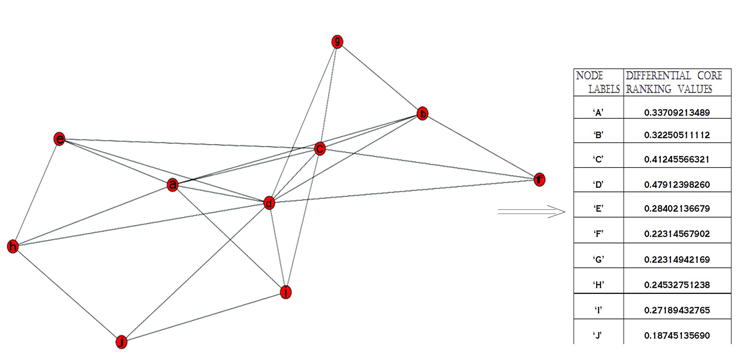
\includegraphics[scale=0.30]{Figures/Mapping_Graph1.jpg}
\caption{Applying Differential Core Ranking, with Betweenness Centrality as the base centrality, to $G_m$.}
\label{gm}
\end{figure}

\begin{figure}[htp]
\centering
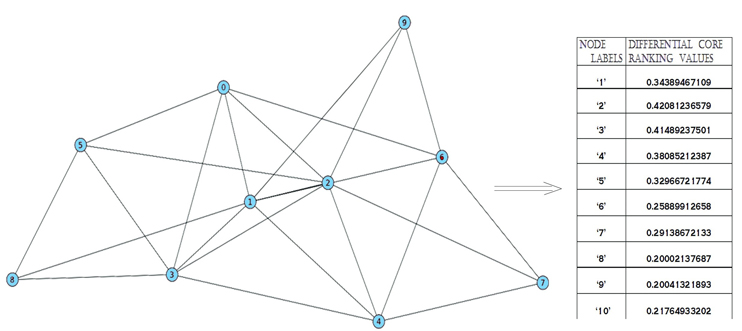
\includegraphics[scale=0.30]{Figures/Mapping_Graph2.jpg}
\caption{Applying Differential Core Ranking, with Betweenness Centrality as the base centrality, to one of the $S_i : 1 \le i  \le \alpha$.}
\label{si}
\end{figure}


\begin{figure}[htp]
\centering
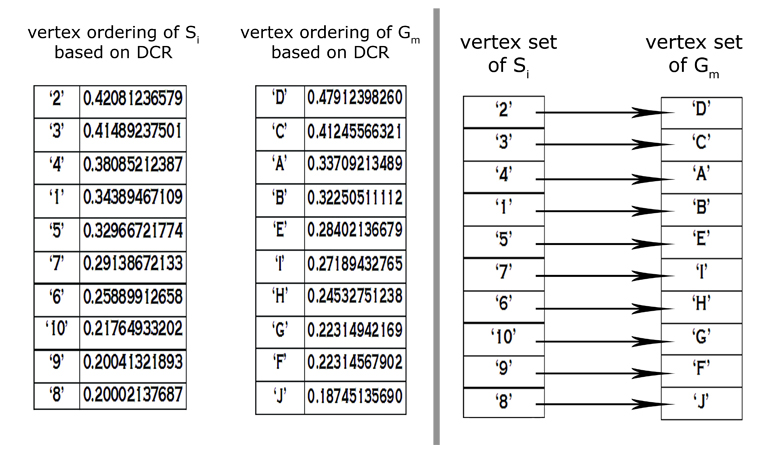
\includegraphics[scale=0.30]{Figures/Mapping_combined.jpg}
\caption{The diagram to the left indicates the vertex ordering based on decreasing Differential Core Ranking for $V_{G_m}$ and $V_{S_i}$. The one on the right shows a direct bijection mapping of vertices between Lists.}
\label{li}
\end{figure}

\begin{figure}[htp]
\centering
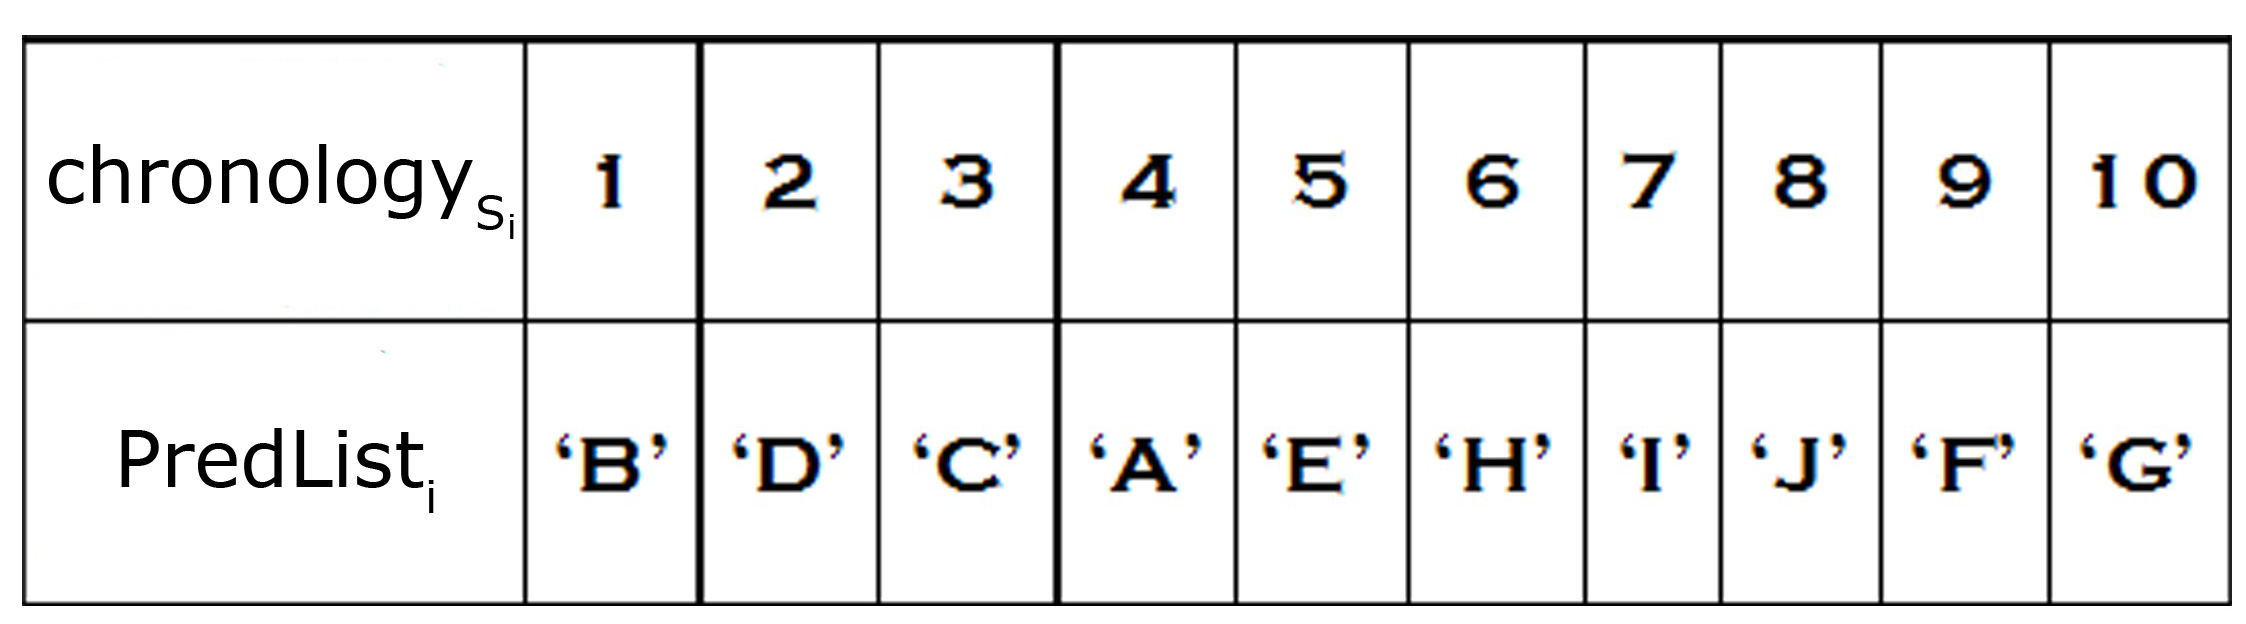
\includegraphics[scale=0.07]{Figures/Mapping_Predicted2.png}
\caption{Deduction of $PredList_i$ by reordering the nodes of $V_m$ according to $chronology_{S_i}$.}
\label{ar}
\end{figure}

\subsection{Analysis of Prediction Lists and Construction of Directed Graph}
\label{DGconstruction}
In the previous section, we have deduced $\alpha$ number of Prediction Lists,  $PredList_i : 1 \le i \le \alpha$. For every pair of vertices $(u,v)$ 
% : u,v \in V_{G_m}$
, we find the order of occurrence of $u$ and $v$ in each $PredList_i$. Let $P_{(u,v)}$ denote the probability of $u$ arriving before $v$ during the inception of $G_m$. We compute $P_{(u,v)}$ as the fraction of the number of times $u$ has occurred before $v$ in the $\alpha$ Prediction Lists. 
% By intuitive reasoning, it is not hard to infer that, if $P_{(u,v)} < 0.5$, then $v$ has probably arrived before $u$ during the inception of $G_m$. Hence, we set $P_{(v,u)} = 1 - P_{(u,v)}$. 
We then construct a Directed Graph $DG$ with vertex set $V_{DG} = V_m$, and an initial edge set $E_{DG}=\phi$. A directed edge from $u$ to $v$ in $DG$ indicates that $u$ has arrived before $v$ during the construction of $G_m$.\\ 

For a pair of vertices $(u,v)$:\\
  if $P_{(u,v)} > 0.5$, then we say that $u$ has arrived before $v$ with a probability $P_{(u,v)}$. We put a directed edge from $u$ to $v$ with a weight $P_{(u,v)}$.\\
  if $P_{(u,v)} < 0.5$, then we say that $v$ has arrived before $u$ with a probability $1 - P_{(u,v)}$. We put a directed edge from $v$ to $u$ with a weight $1 - P_{(u,v)}$.
  
% The algorithm to deduce $DG$ is presented below:\\
% \begin{algorithmic}
%   \STATE Let $S \leftarrow \{S_1,S_2,S_3, ... S_{\alpha}\}$ denote the set of Synthetic Networks
%   \STATE Let $PredList_i$ denote the Prediction List corresponding to $S_i : 1 \le i \le \alpha$ [Refer to algorithm in section (5.2)]
%   \STATE Construct a Directed Graph $DG_m$ with $V_{DG_m} = V_m$ and $E_{DG_m} = \phi$
%   \STATE Let $P_{(u,v)}$ be the probability associated with $(u,v) : u,v \in V_{DG_m}$ in determining if $u$ has come before $v$.
%   \FOR {all unordered pairs $(u,v) : u,v \in V_m\ and\ u \ne v$}
%     \STATE $count \leftarrow 0$
%     \FOR {$i \leftarrow 1\ to\ \alpha$}
%       \IF {$index_{S_i}(u) < index_{S_i}(v)$}
% 	\STATE $count \leftarrow count + 1$
%       \ENDIF
%     \ENDFOR
%     \STATE $P_{(u,v)} \leftarrow count/\alpha$
%     \IF{$P_{(u,v)} > 0.5$}
% 	\STATE append $(u,v)$ to $E_{DG_m}$ with a weight $P_{(u,v)}$
%     \ELSE
% 	\STATE append $(v,u)$ to $E_{DG_m}$ with a weight $1-P_{(u,v)}$
%       \ENDIF
%    \ENDFOR
% \end{algorithmic}

% In the next section, we analyze $DG$ to obtain final predicted order of arrival of nodes in $V_{G_m}$.

\subsection{Transformation of Directed Graph and Node Binning}
\label{nodeBinning}
In this section, we process $DG$ obtained from the previous section to deduce the final prediction of order of arrival of nodes in $G_m$. 
But there is a fair possibility that $DG$ can be a cyclic graph, which can make the prediction order ambiguous. Hence we intend to transform it into a Directed Acyclic Graph (DAG).

% The algorithm to transform $DG$ into $DAG$ is presented below:
\begin{algorithmic}
\STATE Input: Directed Graph $DG$.
\STATE Output: Directed Acyclic Graph $DAG$.
\WHILE {$DG$  contains cycles}
  \STATE Remove the edge $(u,v)$ with the least $P_{(u,v)}$ : $(u,v) \in E_{DG}$. 
\ENDWHILE
\end{algorithmic}

%  $InDegree(v)$ represents the number of nodes that have been predicted to arrive after the arrival of $v$. 
 Ideally, the node that had arrived earliest should have zero in-degree. The next earliest node should have an in-degree equal to 1 and so on. Since we are probabilistically simulating the growth environment of $G_m$, this is not the case.\\
%  it is practically impossible for the nodes to have the same sequence of InDegree as that of their order of arrival.\\

In the final step binning, we will find all the vertices $v$ in $DAG$ having the least in-degree 
% $InDegree(v)$ 
and bunch them into a bin. The binned vertices are hypothesized to have arrived first and are removed from $DAG$. Later we iterate this process over till there are no nodes left in $DAG$. We obtain Final predicted bin ordering.
    
Algorithm to bin the nodes from $DAG$ is presented below:

\begin{algorithmic}
\STATE Input: Directed Acyclic Graph $DAG$
\STATE Output: Bin Ordering
\STATE $count \leftarrow 1$ 
\WHILE {$|V_{DAG}| \neq 0$}
  	\STATE $minInDeg \leftarrow arg\ min (InDegree(u))\ where\ u \in V_{DAG}$
	\STATE Let $B_{count} \leftarrow \{u : \forall u \in V_{DAG}$\\ 
\hspace{1.2in}$and\ InDegree(u) = minInDeg\}$
	\STATE Remove all the nodes in $B_{count}$ from $V_{DAG}$\\
\hspace{1.2in}i.e, $V_{DAG} \leftarrow V_{DAG} - B_{count}$
	\STATE $Count \leftarrow Count + 1$ 
\ENDWHILE
\STATE Let $binOrdering \leftarrow [ B_1, B_2, B_3,...B_{Count}]$
\end{algorithmic}

$binOrdering$ gives the predicted chronological sequence of bins. The accuracy of this prediction, in contrast with accuracy of prediction using centrality measures, is discussed in the next section.

\section{Results and Discussions}
\subsection{Comparison between the predictions from Differential Core Ranking and Plain Centrality}
Let $\chi$ be a base centrality measure. 
Let $Plain\chi_{G_m}$ denote the vertex ordering in the descending order of their $\chi$ centrality values.
% The vertices in the network are arranged in the descending order of their $\chi$ centrality indices. Let this ordering of the nodes be denoted by $Plain\chi_{G_m}$. 
We apply DCR, with the same centrality $\chi$ as the base centrality, to the network $G_m$. 
Let $Differential\chi_{G_m}$ denote the vertex ordering in the descending order of their DCM values.\\
% The vertices in the network are arranged in the descending order of their DCR values. Let this ordering of the nodes be denoted by $Differential\chi_{G_m}$.

$list_{true}$ denotes the actual order of arrival of nodes in $G_m$ (section~\ref{reference_network}). Let the predicted order be denoted by $list_{pred}$. To compute the accuracy of our prediction, we define a new quality measure called $\eta(list_{true},\  list_{pred})$.

\begin{center}
$\eta(list_{true}, list_{pred}) = \frac{ n_c }{^{|V_{G_m}|}C_2}$
\end{center}

where $n_c$ is the number of pairs in $list_{pred}$ that are in correct relative order with respect to $list_{true}$.
To compare the prediction accuracy for the lists $Plain\chi_{G_m}$ and $Differential\chi_{G_m}$, we just compare the values of $\eta(list_{true}, Plain\chi_{G_m})$ and $\eta(list_{true}, Differential\chi_{G_m})$. In our experiments we consider the cases where $\chi$ represents Degree Centrality and Betweenness Centrality.\\

%The figures [10 to 12] represent the plots used to compare the values of $\eta(list_{true}, Plain\chi_{G_m})$ and $\eta(list_{true}, Differential\chi_{G_m})$ for varying number of nodes. Note that the number of connections $C_m$ is kept constant. The red line indicates the $\eta$-measure using Differential Core Centrality, with $\chi$ as the base centrality. The blue line indicates the $\eta$-measure obtained using plain $\chi$ centrality. The x-axis represents the number of nodes. The y-axis denotes $\eta(list_{true}, Differential\chi_{G_m})$ and $\eta(list_{true}, Plain\chi_{G_m})$. In each of the plots, the choice of $\chi$ varies accordingly.

% We now run the  exeperiment on BA networks with 1000 nodes and varying number of connections. The results are depicted in figures [13 to 15]. The x-axis represents the number of connections. The y-axis denotes\\
% $\eta(list_{true}, Differential\chi_{G_m})$ and $\eta(list_{true}, Plain\chi_{G_m})$. In each of the plots, the choice of $\chi$ varies accordingly.

\begin{figure}[htp]
\centering
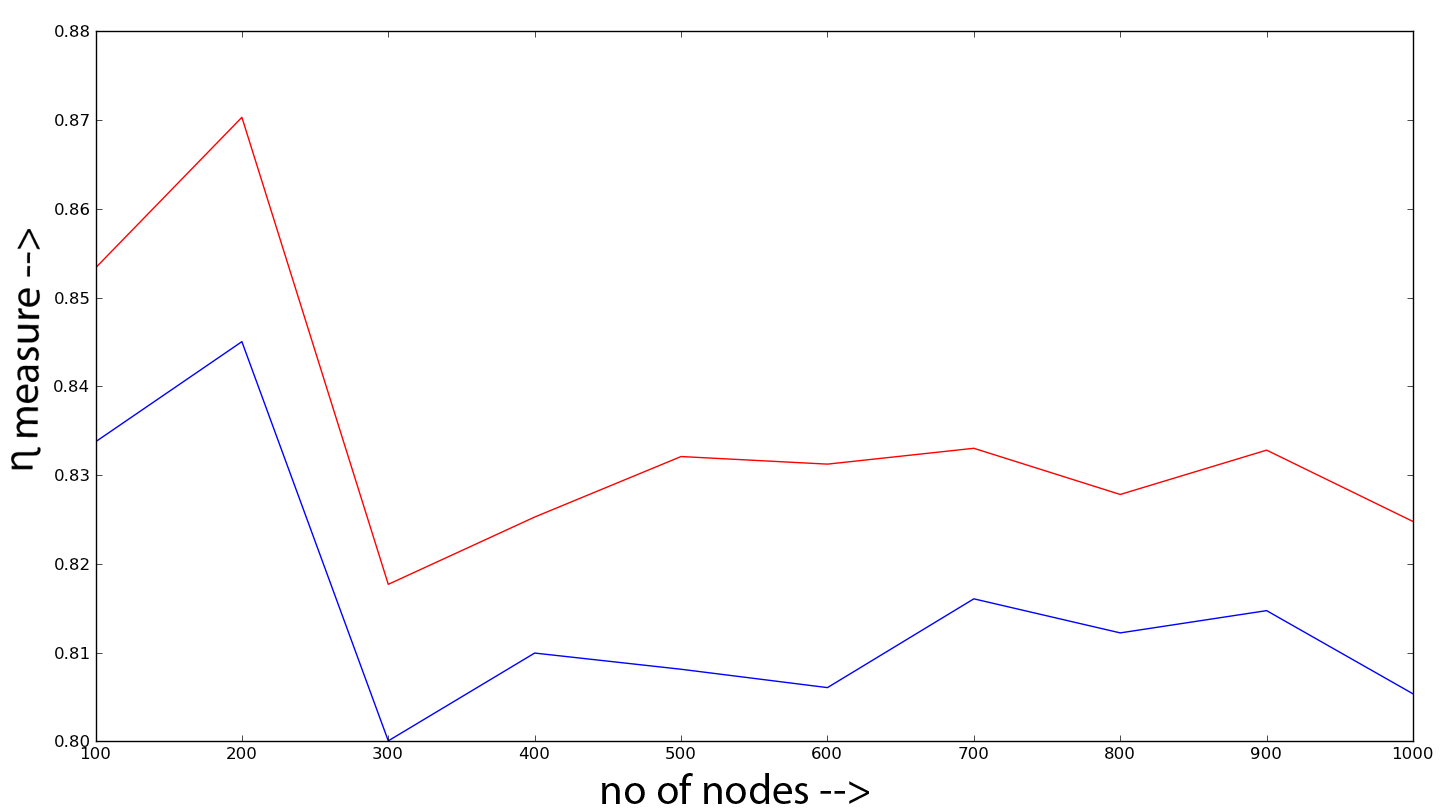
\includegraphics[scale=0.1]{Figures/100_to_1000_nodes_3_connections_degree.png}
\caption{Plot representing the comparision of values of $\eta(list_{true}, Plain\chi_{G_m})$ (blue plot) and $\eta(list_{true}, Differential\chi_{G_m})$ (red plot) for varying number of nodes with $\chi$ : Degree Centrality}
\label{}
\end{figure}

\begin{figure}[htp]
\centering
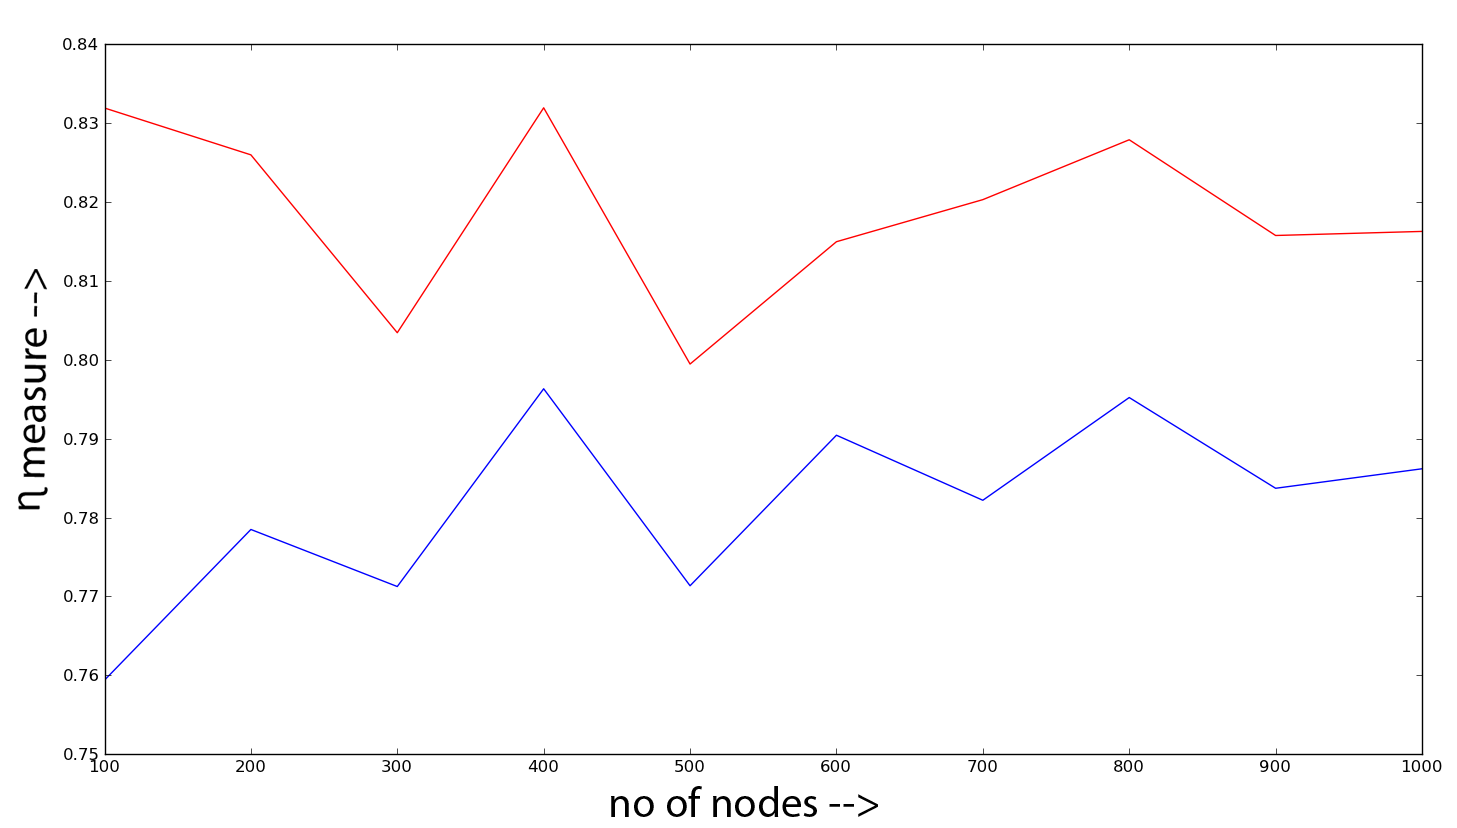
\includegraphics[scale=0.1]{Figures/100_to_1000_nodes_3_connections_betweenness.png}
\caption{Plot representing the comparision of values of $\eta(list_{true}, Plain\chi_{G_m})$ (blue plot) and $\eta(list_{true}, Differential\chi_{G_m})$ (red plot) for varying number of nodes with $\chi$ : Betweenness Centrality}
\label{betweenness}
\end{figure}


% \begin{figure}[htp]
% \centering
% 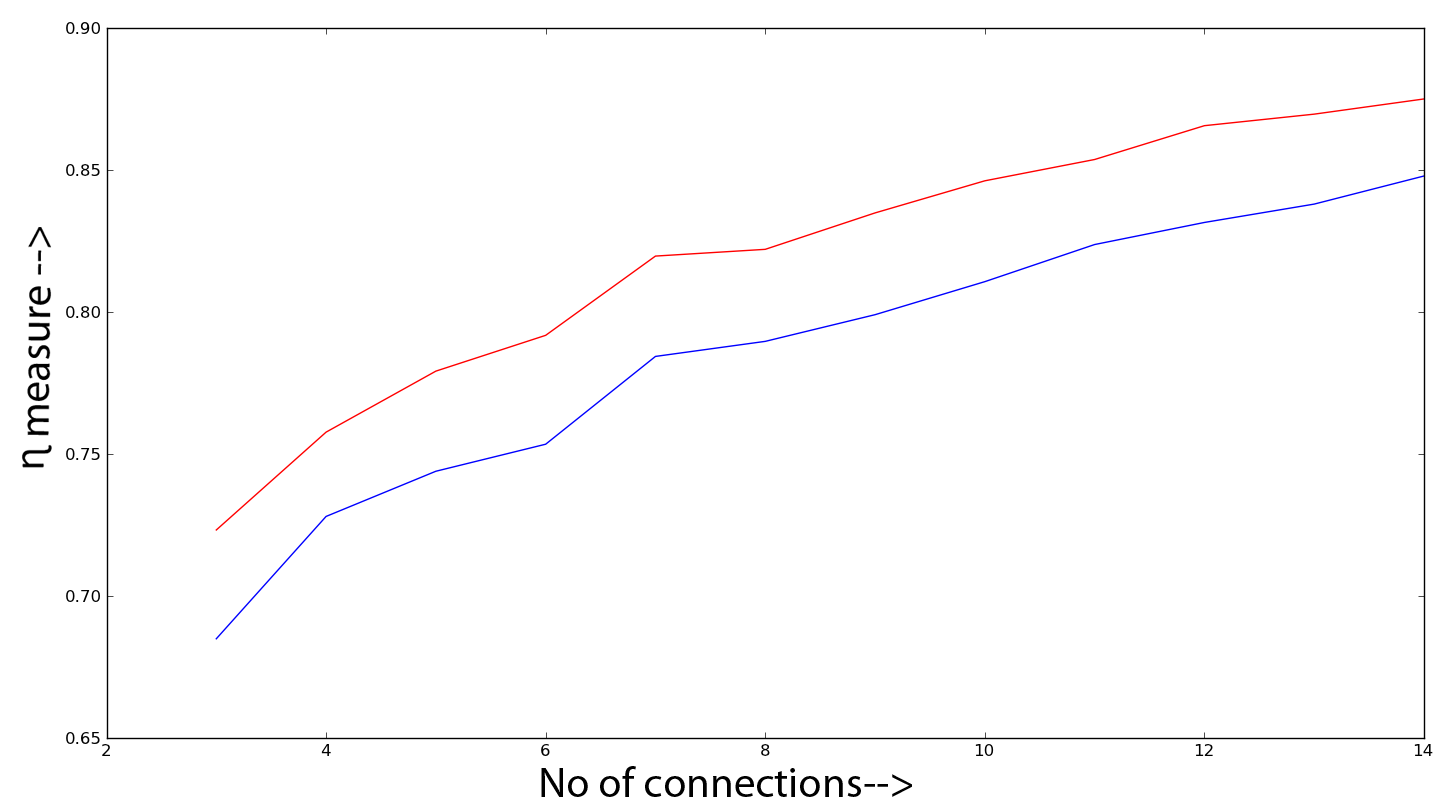
\includegraphics[scale=0.12]{Figures/1000_nodes_3_to_15connections_eigen.png}
% \caption{$\chi$ : Eigen Vector Centrality}
% \label{}
% \end{figure}


%Figures 11 - 13 illustrate the performance of our alogrithm in comparison with the centrality based binning, for varying number of nodes in $G_m$. Figures 14-16 illustrate the performance of our algorithm in comparision with centrality based binning, for varying connection $C_m$ in $G_m$.

\subsection{Prediction of arrival order in every node pair with an attached probability} 

% The outcome of section~\ref{DGconstruction} is a weighted directed graph $DG$. We have associated a probability $P_{(u,v)}$ with every directed edge $(u,v) \in E_G$. $P_{(u,v)}$ indicates the probability with which $u$ has arrived before $v$. From the construction mechanism of $DG$, it is clear that $P_{(u,v)} > 0.5$. Closer the value of $P_{(u,v)}$ to 0.5, harder it is to ascertain the chronological ordering of $u$ and $v$. Note that there is a fair possibility that $DG$ can contain cycles. We claim that the inconsistencies in the prediction might be caused due to edges with $P_{(u,v)}$ close to 0.5. This may lead to a formation of cycles. 

We now present the analytical results that we have obtained, considering $G_m$ as reference network. We have generated $G_m$ using a BA model with 1000 nodes and 3 connections. We generate 50 synthetic networks. So, we set $\alpha = 50$. The analytical results thus obtained is given below:

\begin{figure}[htp]
\centering
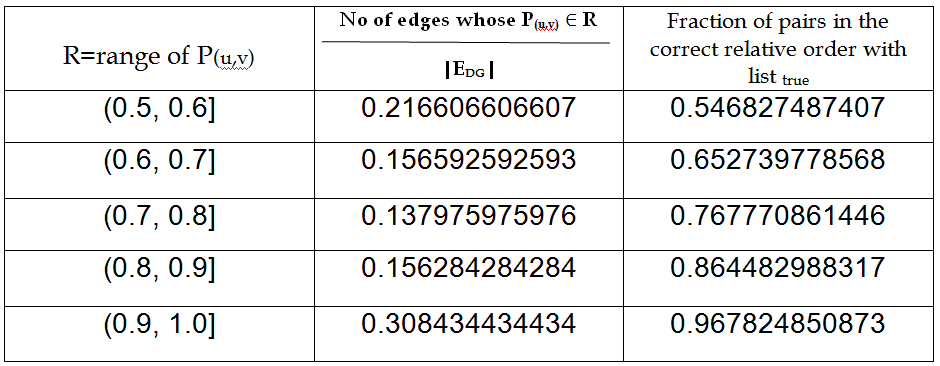
\includegraphics[scale=0.25]{Figures/table.png}
\label{}
\end{figure}

Statistically, from the above table, we observe that the edges $(u,v)$ having $P_{(u,v)}$ in $(0.5, 0.6]$ constitute around 20\% of the edges. We also note that only around 50\% of these edges are in the correct relative order with $list_{true}$. Since a large fraction of edges belonging to this range are in incorrect relative ordering, they contribute to the cycle formation. Cycles introduce inconsistencies in node arrival order, hence they have to be removed. From our experiments, we have found out that $DG$ will become acyclic when we remove the edges $(u,v)$ continually in the increasing order until $P_{(u,v)} \approx 0.6$. We implement the same technique in section~\ref{nodeBinning} to transform $DG$ to $DAG$.\\

Based on the facts and figures from the table, we observe that the fraction of pairs that are in correct relative order with $list_{true}$ increases as the sampled range increases. Hence we conclude that, higher $P_{(u,v)}$ implies a stronger notion of relative ordering of $(u,v)$.

\subsection{Comparison between the predictions from DCR binning and Plain Centrality binning}
The end result of our method (section~\ref{nodeBinning}) is the ordering of the bins, referred to as $binOrdering_{DCR\chi}$. Let $\eta_{DCR\chi}$ denote the BQM score of $binOrdering_{DCR\chi}$, where $\chi$ refers to the base centrality measure for DCR.\\

Let $binOrdering_\chi$ denote the chronology of bins with $\chi$ as the base centrality.
% We derive the $binOrdering_\chi$ with $\Delta$ number of bins, and $\chi$ indicating the centrality measures. 
$binOrdering_{betweenness}$, $binOrdering_{eigen}$ and  $binOrdering_{degree}$ denote the chronology of bins with $\chi$ set as Betweenness, Eigenvector and Degree Centralities respectively.\\

Let $\eta_{betweenness}$, $\eta_{eigen}$ and $\eta_{degree}$ denote the BQM scores of $binOrdering_{betweenness}$, $binOrdering_{eigen}$ and  $binOrdering_{degree}$ respectively. Finally, we compare $\eta_{betweenness}$, $\eta_{eigen}$, $\eta_{degree}$ and $\eta_{DCR\chi}$ where $\chi$ is the base centrality (refer section 4).\\

We perform the above said experiment multiple times for the reference graphs $G_m$ of 1000 nodes and 3 connections. In our experiment, we have set $\alpha = 50$. For each experiment, we choose different base centralities and different $G_m$. We observe that the DCR method yields more accurate results compared to any other plain centrality based approaches. Figures ~\ref{res1} and ~\ref{res2} represents two of those instances and denotes the BQM scores for various binning methodologies.

\begin{figure}[htp]
\centering
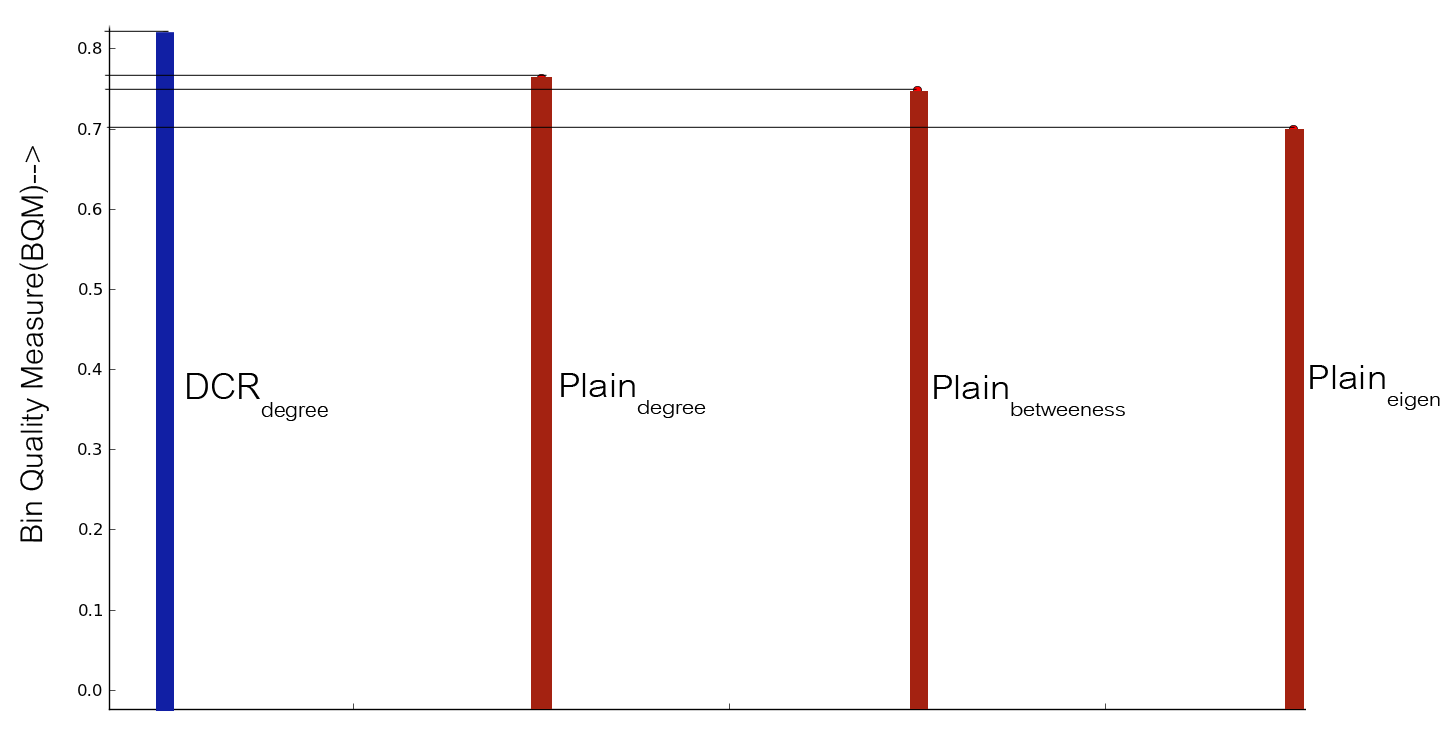
\includegraphics[scale=0.12]{Figures/degree.png}
\caption{$\eta_{DCR_{degree}}=0.804513946531$, 
$\eta_{degree}=0.767615011251$, 
$\eta_{betweenness}=0.759827243464$, 
$\eta_{eigen}=0.695466553648$,
number of bins=91}
\label{res1}
\end{figure}

% \begin{figure}[htp]
% \centering
% 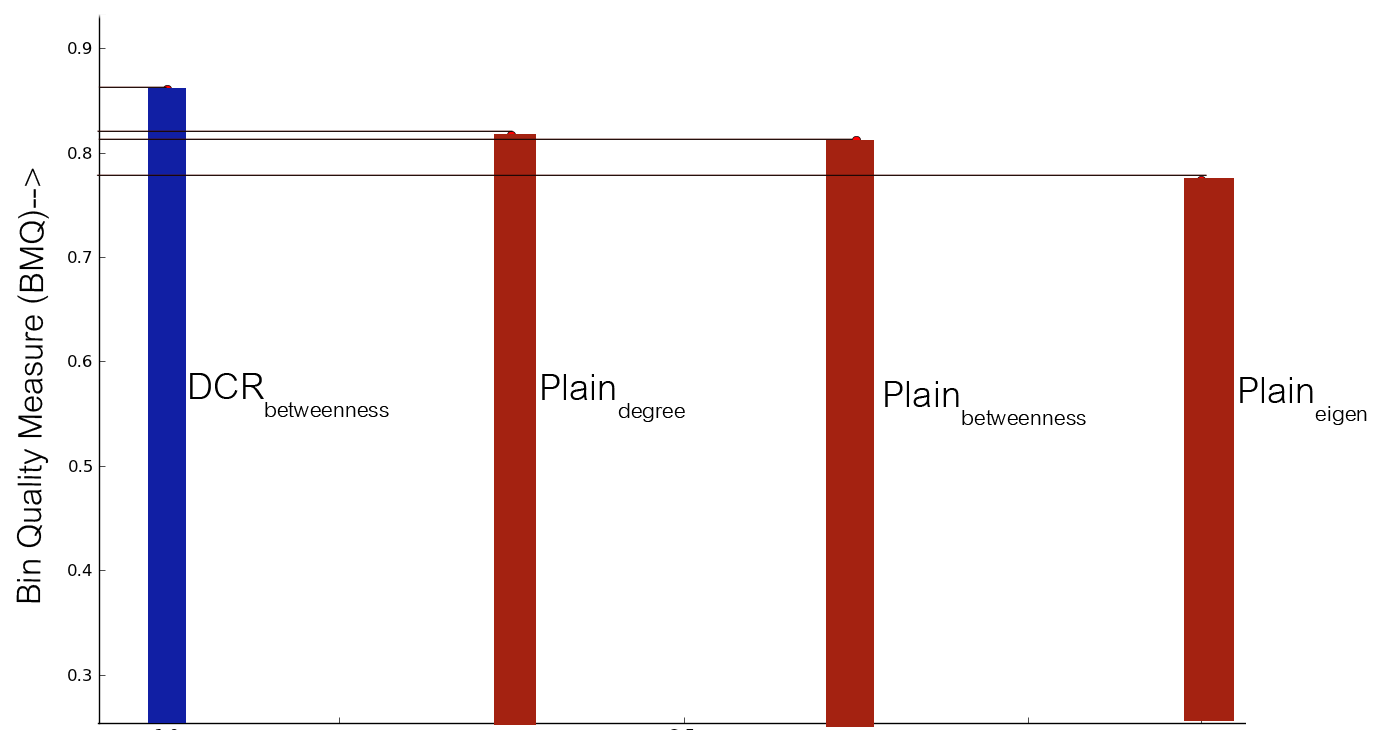
\includegraphics[scale=0.1]{Figures/betweenness.png}
% \caption{$\eta_{DCR_{betweenness}}=0.87153926121$, 
% $\eta_{degree}=0.8251012352$, 
% $\eta_{betweenness}=0.8158246115$, 
% $\eta_{eigen}=0.7823167778$, 
% number of bins=63}
% \label{}
% \end{figure}

\begin{figure}[htp]
\centering
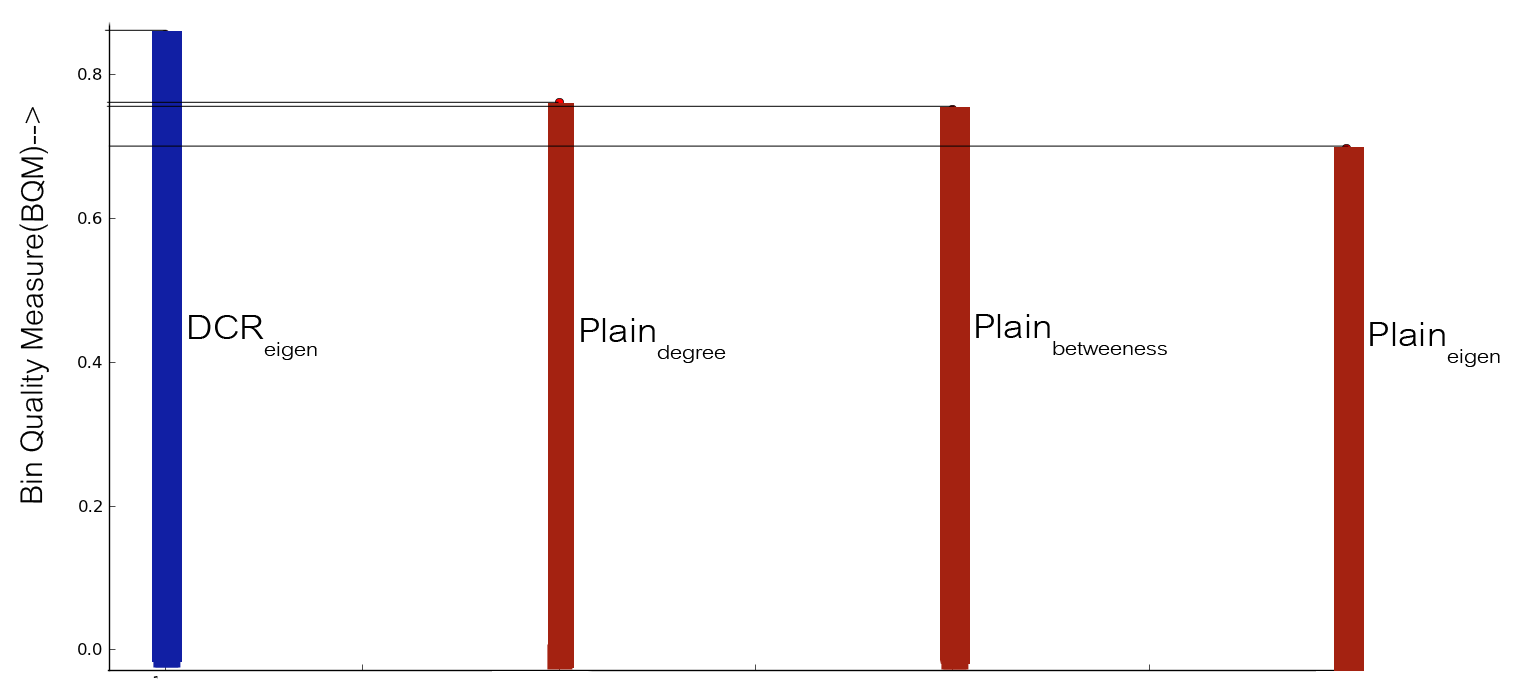
\includegraphics[scale=0.12]{Figures/eigen.png}
\caption{$\eta_{DCR_{eigen}}=0.84654821986$, 
$\eta_{degree}=0.7697124538121$,  
$\eta_{betweenness}=0.753169421166$, 
$\eta_{eigen}=6899122714632$, 
number of bins=77}
\label{res2}
\end{figure}

\section{Conclusion}

We presented a novel framework for uncovering the precursor of a SFN evolved by BA model. Our approach involves the synthesis of many such SFNs, mapping these SFNs with the reference network based on $DCR$ score associated with the nodes and arriving at the final prediction order. We presented 3 results. 1. $DCR$ based prediction, which proved to provide better predicted node arrival results than any other centrality based approaches. 2. Arrival order of every pair of nodes in a SFN, with an associated probability. We empirically proved that most of the node pairs with high probability indeed arrived in the order that we predicted. 3. We also proved that $DCR$ based prediction, when applied in conjunction with the binning methodologies, offered a better accuracy compared to any other plain centrality based approaches.

\bibliographystyle{plain}  
\bibliography{references}

% that's all folks
\end{document}